\documentclass[tikz,border=10pt]{standalone}
\usepackage{tikz}
\usetikzlibrary{positioning}
\usetikzlibrary{shapes.geometric}% tikz node 形状的库
\usetikzlibrary{patterns}
\usepackage{tikz-feynman}
\begin{document}

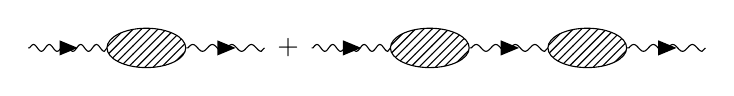
\begin{tikzpicture}[scale=1]
	\begin{feynman}
		%% fig a
		\vertex (a1) at (0,0);
		\vertex[above right = 0 and 1 of a1] (a2);
		\node[draw,pattern=north east lines,shape=ellipse,minimum width=1cm ,minimum height=.5cm,anchor=center] (a3) at (1.5,0);
		\vertex[above right = 0 and 3 of a1] (a4);
		% 对各个顶点连线
		\diagram*{
		(a1) --[charged boson] (a2);
		(a3) --[charged boson] (a4);
		};
	\end{feynman}
	\node at (3.3,0) {$+$};
	\begin{feynman}[xshift=3.6cm]
		%% fig a
		\vertex (b1) at (0,0);
		\vertex[above right = 0 and 1 of b1] (b2);
		\node[draw,pattern=north east lines,shape=ellipse,minimum width=1cm ,minimum height=.5cm,anchor=center] (b3) at (1.5,0);
		\vertex[above right = 0 and 3 of b1] (b4);
		\node[draw,pattern=north east lines,shape=ellipse,minimum width=1cm,minimum height=.5cm,anchor=center] (b5) at (3.5,0);
		\vertex[above right = 0 and 5 of b1] (b6);
		% 对各个顶点连线
		\diagram*{
		(b1) --[charged boson] (b2);
		(b3) --[charged boson] (b4);
		(b5) --[charged boson] (b6);
		};
	\end{feynman}
\end{tikzpicture}

\end{document}